%                                                                 aa.dem
% AA vers. 9.1, LaTeX class for Astronomy & Astrophysics
% demonstration file
%                                                       (c) EDP Sciences
%-----------------------------------------------------------------------
%
%\documentclass[referee]{aa} % for a referee version
%\documentclass[onecolumn]{aa} % for a paper on 1 column  
%\documentclass[longauth]{aa} % for the long lists of affiliations 
%\documentclass[letter]{aa} % for the letters 
%\documentclass[bibyear]{aa} % if the references are not structured 
%                              according to the author-year natbib style

%
\documentclass{aa}  

%
\usepackage{graphicx}
%%%%%%%%%%%%%%%%%%%%%%%%%%%%%%%%%%%%%%%%
\usepackage{txfonts}
%%%%%%%%%%%%%%%%%%%%%%%%%%%%%%%%%%%%%%%%
%\usepackage[options]{hyperref}
% To add links in your PDF file, use the package "hyperref"
% with options according to your LaTeX or PDFLaTeX drivers.
\usepackage[colorlinks=true,citecolor=blue,linkcolor=blue]{hyperref}
% To add links in your PDF file, use the package "hyperref"
% with options according to your LaTeX or PDFLaTeX drivers.
%
\usepackage{natbib}
\bibpunct{(}{)}{;}{a}{}{,} % to follow the A&A style
%\usepackage{enumitem}
\usepackage{bm}
\usepackage{upgreek}
\usepackage[dvipsnames]{xcolor}
\usepackage{amsmath}    % Advanced maths commands
%\usepackage{amssymb}
%
\begin{document} 


   \title{Lens models of galaxy--galaxy strong lenses}

   \subtitle{}

   \author{BDLensing team
          \inst{1}
          \and
          C. Ptolemy\inst{2}\fnmsep\thanks{Just to show the usage
          of the elements in the author field}
          }

   \institute{Institute for Astronomy (IfA), University of Vienna,
              T\"urkenschanzstrasse 17, A-1180 Vienna\\
              \email{wuchterl@amok.ast.univie.ac.at}
         \and
             University of Alexandria, Department of Geography, ...\\
             \email{c.ptolemy@hipparch.uheaven.space}
             \thanks{The university of heaven temporarily does not
                     accept e-mails}
             }

   \date{Received September 15, 1996; accepted March 16, 1997}

% \abstract{}{}{}{}{} 
% 5 {} token are mandatory
 
  \abstract
  % context heading (optional)
  % {} leave it empty if necessary  
   {To investigate the physical nature of the `nuc\-leated instability' of
   proto giant planets, the stability of layers
   in static, radiative gas spheres is analysed on the basis of Baker's
   standard one-zone model.}
  % aims heading (mandatory)
   {It is shown that stability
   depends only upon the equations of state, the opacities and the local
   thermodynamic state in the layer. Stability and instability can
   therefore be expressed in the form of stability equations of state
   which are universal for a given composition.}
  % methods heading (mandatory)
   {The stability equations of state are
   calculated for solar composition and are displayed in the domain
   $-14 \leq \lg \rho / \mathrm{[g\, cm^{-3}]} \leq 0 $,
   $ 8.8 \leq \lg e / \mathrm{[erg\, g^{-1}]} \leq 17.7$. These displays
   may be
   used to determine the one-zone stability of layers in stellar
   or planetary structure models by directly reading off the value of
   the stability equations for the thermodynamic state of these layers,
   specified
   by state quantities as density $\rho$, temperature $T$ or
   specific internal energy $e$.
   Regions of instability in the $(\rho,e)$-plane are described
   and related to the underlying microphysical processes.}
  % results heading (mandatory)
   {Vibrational instability is found to be a common phenomenon
   at temperatures lower than the second He ionisation
   zone. The $\kappa$-mechanism is widespread under `cool'
   conditions.}
  % conclusions heading (optional), leave it empty if necessary 
   {}

   \keywords{giant planet formation --
                $\kappa$-mechanism --
                stability of gas spheres
               }

   \maketitle
%
%-------------------------------------------------------------------

\section{Introduction}

\section{Data}

\subsection{\textit{HST} imaging}

% example https://arxiv.org/pdf/2008.11724.pdf and https://arxiv.org/pdf/1807.09278.pdf

\subsection{Description of special systems (can be finalized later)}

% example in https://arxiv.org/pdf/1807.09278.pdf

\begin{figure*}
	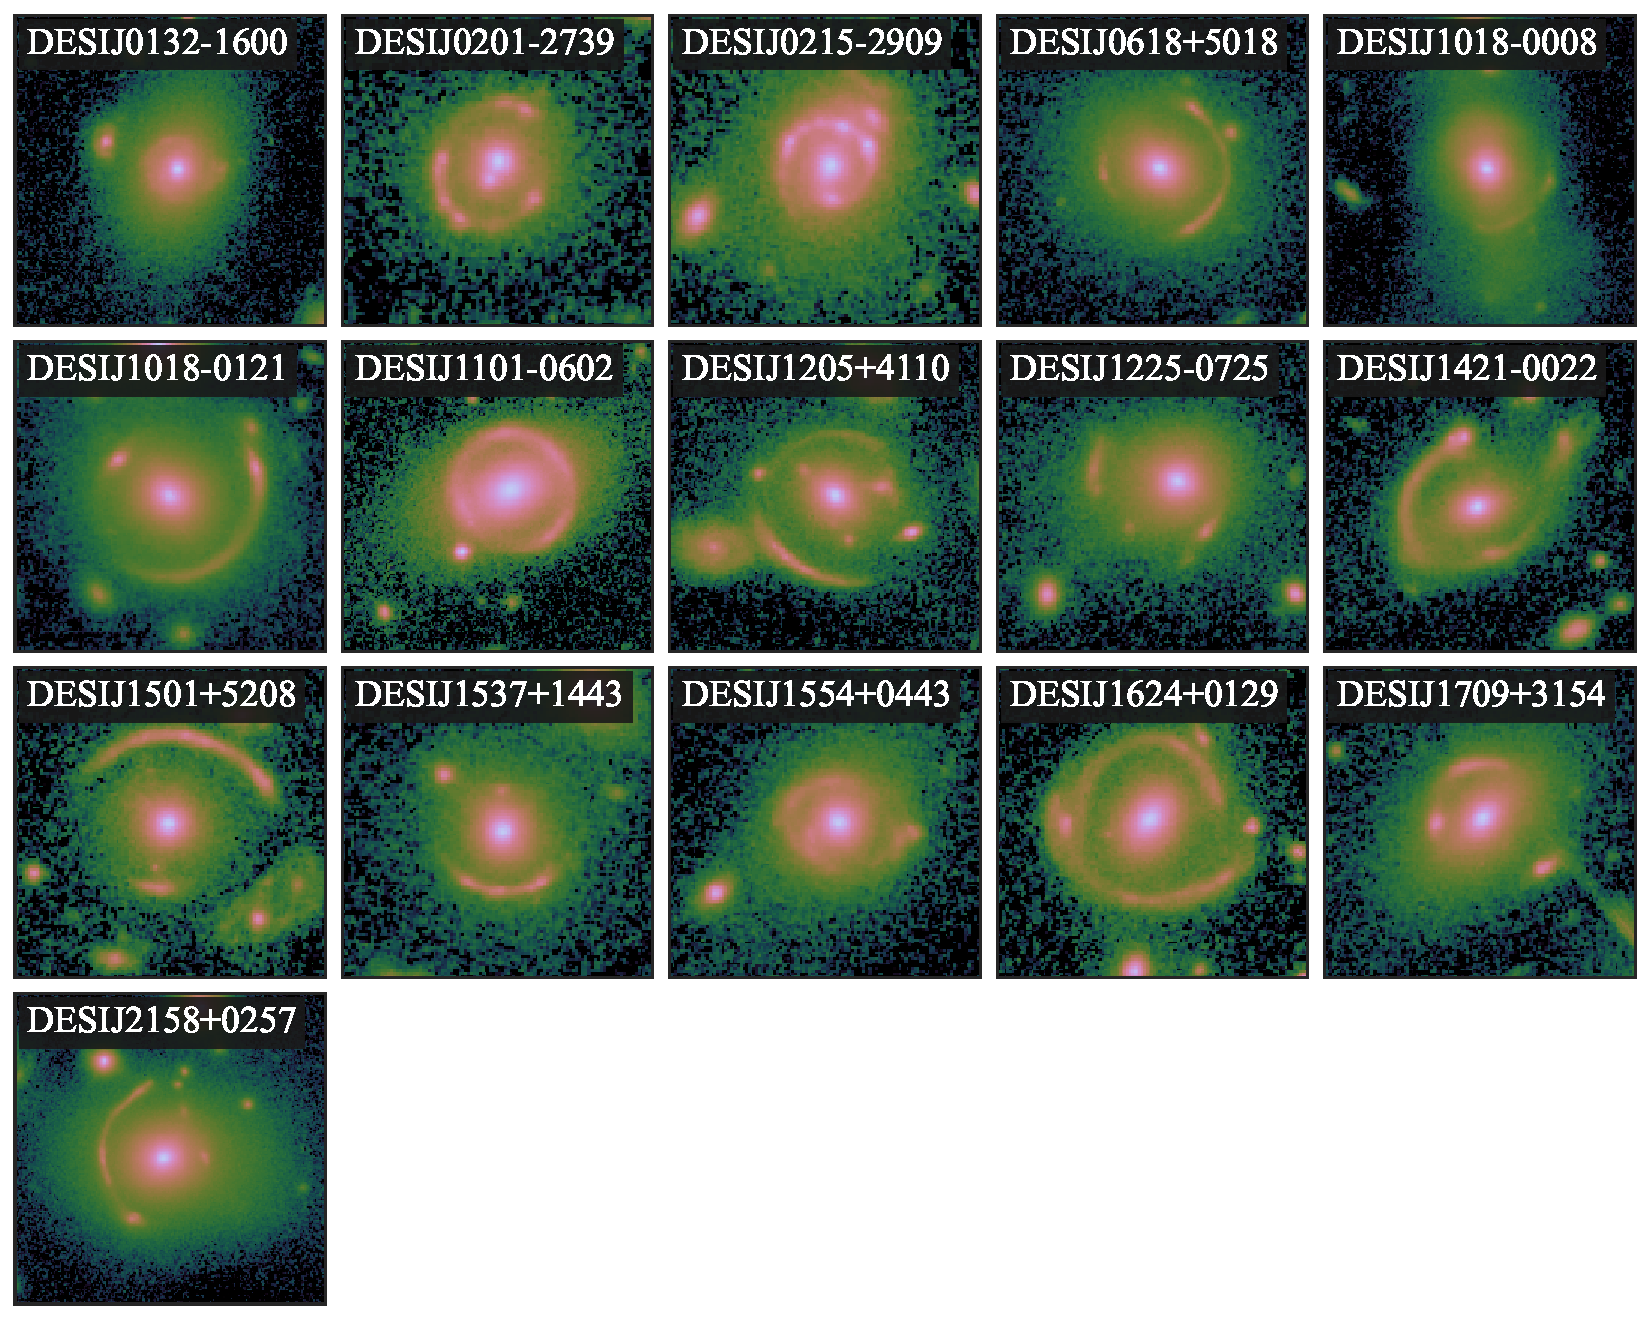
\includegraphics[width=\textwidth]{figures/lens_montage.pdf}
	\caption{\label{fig:montage}
	Montage of all the lens systems.
	}
\end{figure*}

\section{Lens modelling (Method)}

\subsection{Lens model ingredients}

\subsubsection{Mass profile}
% EPL, external shear 
% example https://arxiv.org/pdf/1807.09278.pdf

\subsubsection{Light profiles}
% Sersic or double sersic for lens galaxy

% Sersic + shapelets for source galaxy

\subsection{Modelling procedure}

% description of PSO, MCMC etc.

\section{Result}

\subsection{Lens model parameters}

% need table of model parameters, example https://arxiv.org/pdf/2008.11724.pdf

\subsection{Estimation of $\Sigma_{10}$}

\subsection{Mass and light alignment}

% Pearson correlation coefficient: https://en.wikipedia.org/wiki/Pearson_correlation_coefficient

\section{Discussion and conclusion}

\begin{acknowledgements}
      Part of this work was supported by the German
      \emph{Deut\-sche For\-schungs\-ge\-mein\-schaft, DFG\/} project
      number Ts~17/2--1.
\end{acknowledgements}

% WARNING
%-------------------------------------------------------------------
% Please note that we have included the references to the file aa.dem in
% order to compile it, but we ask you to:
%
% - use BibTeX with the regular commands:
%   \bibliographystyle{aa} % style aa.bst
%   \bibliography{Yourfile} % your references Yourfile.bib
%
% - join the .bib files when you upload your source files
%-------------------------------------------------------------------

% - use BibTeX with the regular commands:
\bibliographystyle{aa} % style aa.bst
\bibliography{ajshajib} % your references Yourfile.bib

\end{document}